
\subsection{Vorstellung der Infrastruktur und Code-Entwicklung (HB)}


\subsubsection{Infrastruktur}

Die für dieses Projekt eingesetzte Infrastruktur setzt auf verschiedene Komponenten, deren Zusammenspiel hier in einer vereinfachten Darstellung zu erkennen ist und im Folgenden näher beschrieben wird: 

\begin{figure}[H]
    \centering
    \label{fig:henning-dia-git-dev-server}
    \caption{Konzept: Entwicklung, Codeverteilung, Produktivnahme}
    \fbox{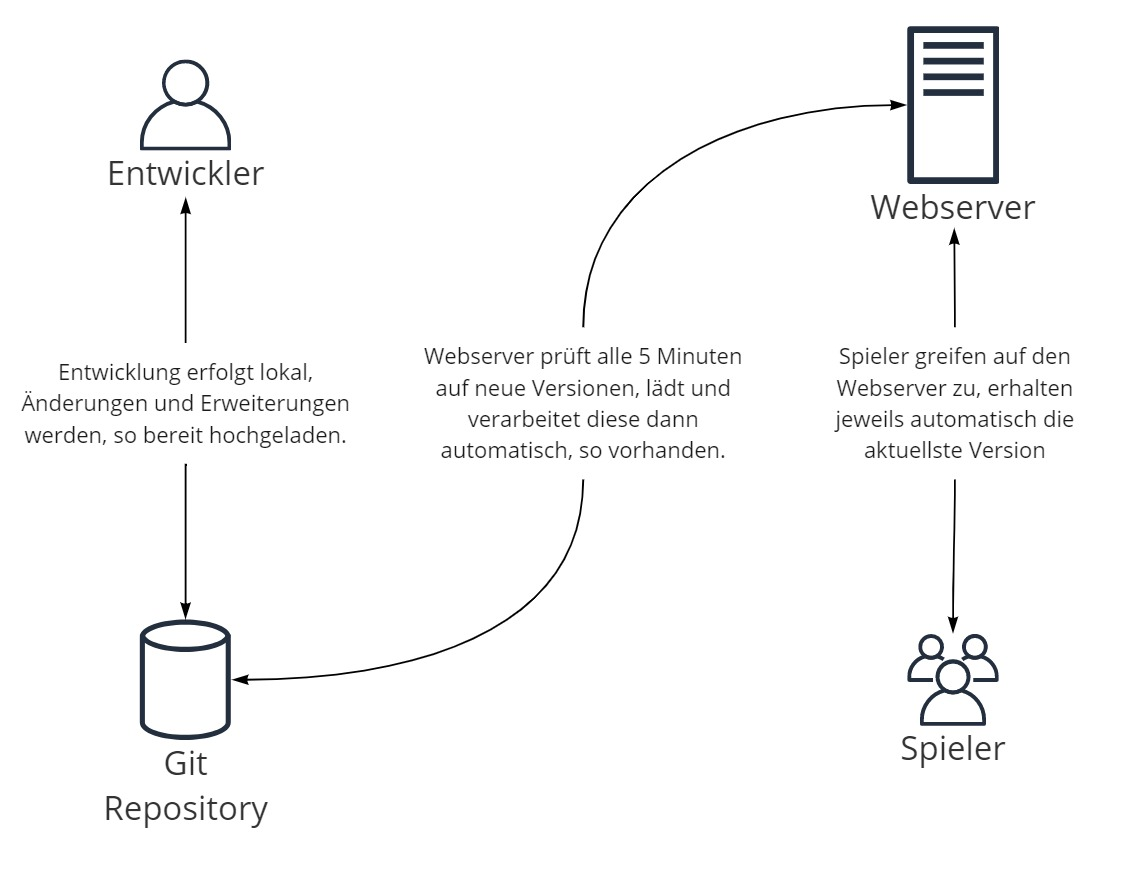
\includegraphics[width=0.8\textwidth]{henning-dia-git-dev-server}}
\end{figure}


Die Dienste selbst laufen auf einem für dieses Projekt bei der \textbf{HostEurope GmbH}\footnote{Siehe \url{https://www.hosteurope.de/Server/Virtual-Server/}.} angemieten, virtuellem Server. Das Produkt nennt sich \enquote{Virtual Server 10.0} und verfügt in der geringsten Austattung über 1 vCPU, 2 GB RAM sowie 40 GB SSD-Speicher. Auf dem Server läuft Debian 11. Der Server hat außerdem eine feste IP-Adresse. Einrichtungskosten gab es keine. Der Vertrag ist montalich kündbar. Der Mietpreis beträgt 5,99 EUR incl. MwSt. monatlich.

Weiter wurde bei \textbf{INWX GmbH}\footnote{Siehe \url{https://www.inwx.de/de/de-domain}.} zu dem Server auch eine Domain gekauft sowie entsprechende Namensservereinträge hinterlegt, die den Betrieb eines Traefik-Proxys mit Subdomains zu Domain erlauben. Auch hier gab es keine Einrichtungskosten. Der Preis für die Domain beträgt pro 5,97 EUR incl. MwSt. pro Jahr. 


Abseites der vorgenannten Hardware, stellt das gemeinsame \textbf{Git-Repository auf Github}\footnote{Siehe \url{https://github.com/tstsrv-de/rpg/}.} einen zentralen Punkt der Infrastruktur dar. In diesem Repository liegen alle Elemente des Projektes: Code, Skripte und Dokumentation.

Die Funktionen des Repositorys sind folgende: \begin{itemize}
    \item Entwickler übermitteln neue Inhalte in das Repository (push).
    \item Entwickler erhalten den stets aktuellen Entwicklungsstand aus dem Repository (pull, fetch).
    \item Der Server lädt neue Inhalte aus dem Repository automatisch und aktualisiert die Dienste.
    \item Alle Beteiligten und auch Dritte können über das Repository die Entwicklung nachvollziehen. 
\end{itemize}


Für den Update-Prozess des Servers und der Dienste wurde ein Cron-Skript erstellt, dass laufend prüft ob neue Commits im Repository vorhanden sind (siehe \textbf{Codelisting 1} unten, Zeile 5). Wenn ja, wird der Django-Webserver gestoppt (Zeile 7), die neuen Inhalte heruntergeladen, verarbeitet und der Django-Webserver im Anschluss wieder gestartet (Zeile 15). 

\textbf{Codelisting 1: \enquote{rpg/server-update-cron.sh}, gekürzt um Logging:}
\begin{lstlisting}[language=bash]
#!/bin/bash
cd /home/rjhadmin/tstsrv/
now=$(date "+%F %H:%M:%S")
git -C /home/rjhadmin/tstsrv/ fetch origin 
if  [ `git -C /home/rjhadmin/tstsrv/ rev-list HEAD...origin/main --count` != 0 ] 
then
    docker-compose --project-directory /home/rjhadmin/tstsrv/ stop rpg  
    git -C /home/rjhadmin/tstsrv/ reset --hard origin/main  
    git -C /home/rjhadmin/tstsrv/ fetch
    git -C /home/rjhadmin/tstsrv/ pull 
    chmod +x /home/rjhadmin/tstsrv/*.sh 
    docker-compose --project-directory /home/rjhadmin/tstsrv/ run rpg python rpg/manage.py makemigrations 
    docker-compose --project-directory /home/rjhadmin/tstsrv/ run rpg python rpg/manage.py migrate 
    docker-compose --project-directory /home/rjhadmin/tstsrv/ run rpg python rpg/manage.py loaddata db_sample_data.json 
    docker-compose --project-directory /home/rjhadmin/tstsrv/ start rpg 
\end{lstlisting}



Ein weiterer wesentlicher Punkt der Software-Infrastruktur ist \textbf{Docker sowie die Container} für den Django-Server, die Datenbank und den Reverse-Proxy. Hier stehen für die lokale Entwicklung \enquote{docker-compose}-Skripte für Windows und auch unixartige Systeme wie Linux und MacOS zur Verfügung. Ebenso für den Betrieb des Servers. Details zur Einrichtung und Nutzung wurden in der \textbf{Readme Repositorys}\footnote{Siehe \url{https://github.com/tstsrv-de/rpg/blob/main/README.md}.} hinterlegt. 


Der Traefik-Proxy wurde so eingerichtet, dass Anfragen auf den Ports HTTP 80 und HTTPS 443 angenommen werden. Anfragen an HTTP 80, werden automatisch umgeleitet an HTTPS 443. Die notwendigen Zertrifikate für die Subdomains werden vollautomatisch vom Traefik-Proxy über Letsencrypt angefordert und verwaltet. Als Grundlage für die Konfiguration diente eine Vorlage von Igor Bubelov\footnote{Siehe Github-Repository dazu \url{https://github.com/bubelov/traefik-letsencrypt-compose}.} die entsprechend um die Funktionen für den Django-Webserver und die Datenbank erweitert wurden.



Die hier entwickelte Konfiguration erweis sich als so verlässlich, dass auch ein anderes Projektteam (\textbf{Deskshare\footnote{Siehe \url{https://github.com/tstsrv-de/deskshare} bzw. \url{https://deskshare.tstsrv.de/}.}}) aus unserem Studiengang, ihre Dienste auf unserer Hardware unter einer eigenen Subdomian betreiben konnte. Die Anbindung an den Traefik-Proxy war möglich, auch die SSL-Zertrifikate wurden vollautomatisch erstelt. Weiter konnte auch des Update-Konzepts mittels Cron-Dienst und Github-Repository übernommen werden, so dass das andere Projektteam eigenständig entwickeln konnte. 


Die Ressourcen des Servers reichen hier für beide Projekte, auch in der Phase vor Abgabe der Arbeiten, aus: 

\begin{figure}[H]
    \centering
    \label{fig:henning-server-auslastung}
    \caption{Bildschirmfoto: Server Auslastung}
    \fbox{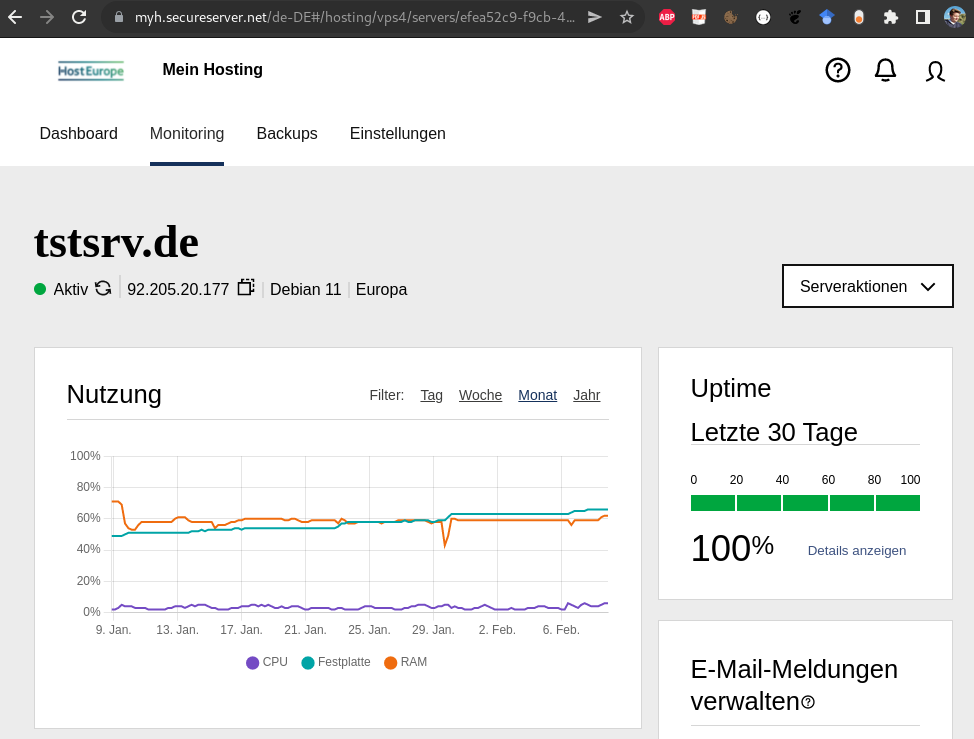
\includegraphics[width=0.8\textwidth]{server-auslastung.png}}
\end{figure}






\subsubsection{Initialisierung der Django-Anwendung}

Nach dem Aufbau der grundsätzlichen Funktionen des Servers (Update-Systemdienste und Cron-Skripte), wurde die Django-Anwendung initialisiert. Der Abaluf orientierte sich hier an den in den Vorlesungen gewonnenen Erkenntnissen und wurde im Anhang (siehe Anhang \ref{django-init}) stichpunktartig festgealten. 

Im Anschluss daran wurden dann zuerst grundlegende Funktionen für die Benutzer-Regeistrierung am System hinzugefügt. Das  insbesondere unter Nutzung von zwei Anleitungen\footnote{Siehe  \url{https://www.nintyzeros.com/2020/06/login-register-user\%20page-in\%20django.html} und \url{https://docs.djangoproject.com/en/3.2/topics/auth/default/\#built-in-auth-forms}.}.


Da das Projekt selbst die Entwicklung eines Spiels umfasste, wurde hier bewusst auf die Implementation von allen ansonsten mit einer Benutzerverwaltung im Zusammenhang stehenden Funktionen verzichtet. Es ist somit \textbf{nicht möglich}, seinen Benutzer z.B. zu löschen oder \textbf{ein vergessenes Passwort} zu erneuern. Unser Fokus lag hier, den Anforderungen entsprechend, auf der Entwicklung der Hauptanwendung. 

Es wird hier in dieser Dokumentation auch nicht weiter auf die implementierte Benutzerverwaltung eingegangen, da es sich um weithin bekannte Standart-Features von Django handelt.

Mit Abschluss der Einrichtung der Django-Anwendung, liegt ein mit den bekannten Funktionen (wie Datenbankmodelle, Benutzerverwaltung, DB-Migrationen, ...) nutzbarer Django-Webserver vor. 
Für die Entwickler und die Entwicklung selbst, ist die direkte Interaktion mit dem Django-Webserver selbst, nicht mehr notwendig. Die entwickelten Skripe, starten den Webserver mit allen notwendigen Paramentern selsbtständig und führen vorher auch notwendige Schritte wie \enquote{makemigrations, migrate oder loaddata} selsbtständig aus. Beispielhaft hier ein Auszug aus dem Skript für den Start der lokalen Entwicklungsumgebung unter unixartigen Betriebssystemen\footnote{Siehe \url{https://github.com/tstsrv-de/rpg/blob/main/local-dev-start.sh}.}: 

\begin{lstlisting}[language=bash]
#!/bin/bash
docker-compose -f local-dev-docker-compose.yml up -d
docker-compose -f local-dev-docker-compose.yml exec rpg python rpg/manage.py makemigrations
docker-compose -f local-dev-docker-compose.yml exec rpg python rpg/manage.py migrate
docker-compose -f local-dev-docker-compose.yml exec rpg python rpg/manage.py loaddata db_sample_data.json
docker-compose -f local-dev-docker-compose.yml stop
docker-compose -f local-dev-docker-compose.yml up 
\end{lstlisting}


\subsubsection{Entwicklung von Grundfunktionen des Spiels}

In der Zeit vom 25.11.2021 bis zum 09.01.2022 wurden von Henning Beier im weiteren das Backend, das Datenbankmodell und die wesentlichen Funktionen des Spiels, entsprechend der in den Projektbesprechungen festgehaltenen Anforderungen, entwickelt.


\begin{figure}[H]
    \centering
    \label{fig:henning-konzept-datenbankmodell}
    \caption{Konzeptionierung: Datenbankmodell}
    \subfloat[Entwurfszeichnung vom 23.11.2021]{\fbox{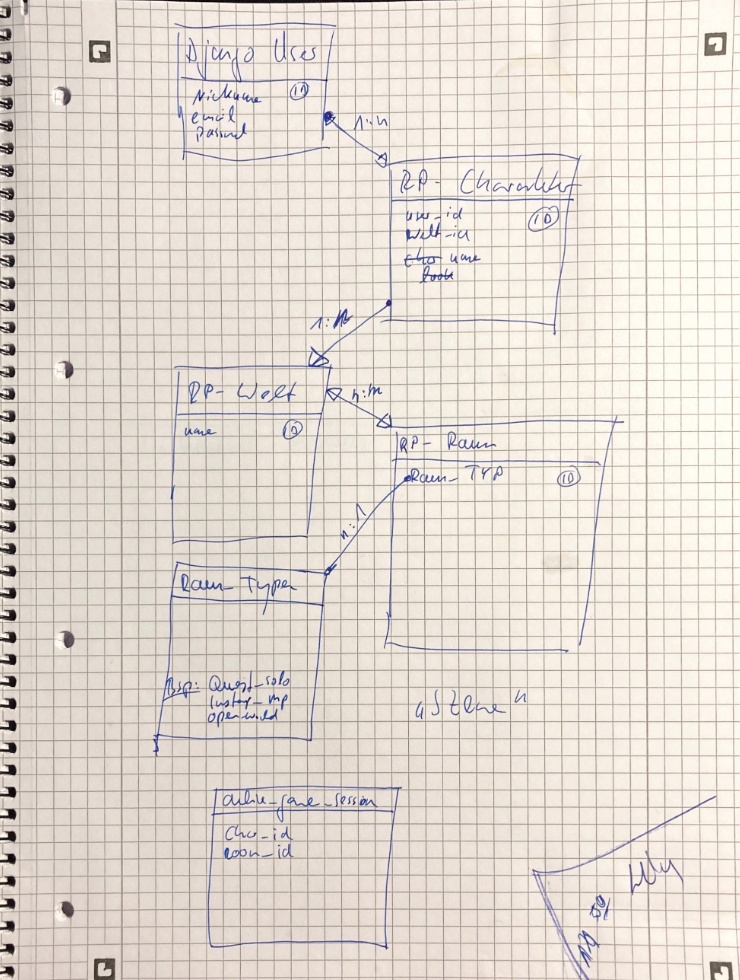
\includegraphics[width=0.5\linewidth]{2021-11-23-erstes-db-konzept}}}
    \subfloat[Weiterentwickelter Entwurf (05.12.2021)]{\fbox{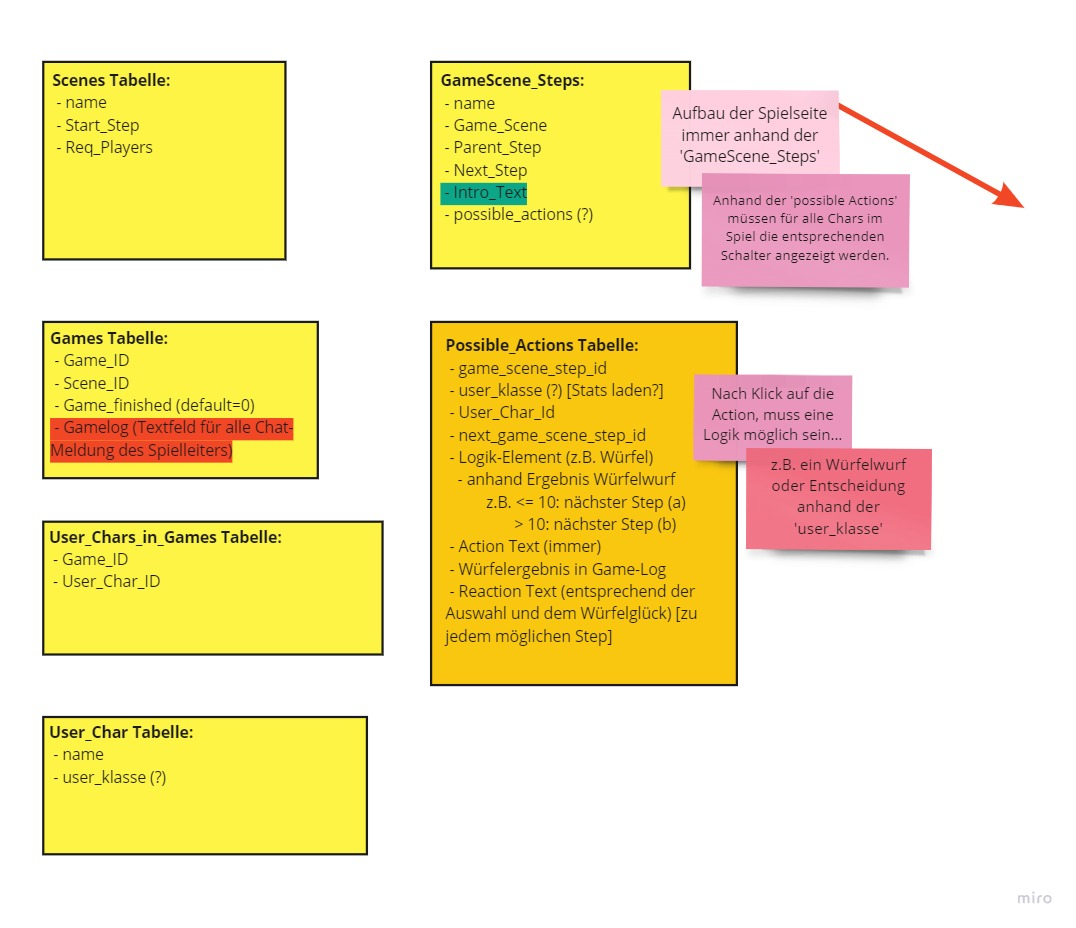
\includegraphics[width=0.5\linewidth]{2021-12-05-Projketbesprechung-Miro-c}}}
\end{figure}



\subsubsection{Code-Entwicklung}
\textbf{Entwicklung, Mittwoch 24.11.2021}

Einbau von Grundlagen: 
\begin{itemize}
    \item Update der Django-Basis Installtion bzw. des Projektes (Commit \url{https://git.io/JSqbt}). 
    \item Auto-Download und restart der Docker-Container bei neuen Commits im Repository auf Github per Cron-Jobjob-Script (siehe \url{https://git.io/JStjW}).
\end{itemize}


\textbf{Entwicklung, Donnerstag 25.11.2021}

Einbau der Charaktere als Datenbank-Modell und View in Django (Commit \url{https://git.io/JSmOd}).



\textbf{Entwicklung, Samstag 27.11.2021}

Einbau der Weltkarte bzw. Levelauswahl (Commit \url{https://git.io/JSmG8}).



\textbf{Entwicklung, Sonntag 28.11.2021}

\begin{itemize}
    \item Einbau einer Web-Sockets Chat-Funktion unter Nutzung einer Anleitung\footnote{Siehe \url{https://github.com/veryacademy/YT-Django-Project-Chatroom-Getting-Started}. } (Commit \url{https://git.io/JSmlS} sowie folgender Commits von diesem Tag).
    \item (Teilweise) Installation der Entwicklungsumgebung, Docker sowie Git bei Julian und Rico sowie jeweils zwei erste Test-Commits incl. anschließendem Auto-Update des Servers (Rico: \url{https://git.io/JSmKV} und Julian: \url{https://git.io/JSmoF}).
\end{itemize}



\textbf{Entwicklung, Montag 29.11.2021}

Erstellung eines Web-Sockets für eine Counter-Funktion incl. der notwendigen Anpassungen an Datenbankmodell, der Django-Reciver und -Consumer (Commit \url{https://git.io/JSmDa}).



\textbf{Entwicklung, Dienstag 30.11.2021}

Einbau einer Lobby und einer Chatfunktion in dieser Lobby -- Jeweils abhängig von der Lobby werden dynamisch Websockets geöffnet (Commits \url{https://git.io/JSm5n} und \url{https://git.io/JSm5N} sowie weitere Anpassungen und Korrekturen in den Commits vom 01.12.2021).


\textbf{Entwicklung, Samstag 04.12.2021}

Flask8 als Code-Linter genutzt und einige Anpassungen entsprechend vorgenommen (Commit \url{https://git.io/JSmN2}).


\textbf{Entwicklung, Sonntag 05.12.2021}

Einbau der Spielseite selbst als logischer Schritte nach der Weltkarte (als Levelauswahl) und der Lobby (Spielfindung /-erstellung) (Commits \url{https://git.io/JSYLS}, \url{https://git.io/JSYqd} und \url{https://git.io/JSYmV}).



\textbf{Entwicklung, Sonntag 12.12.2021:}

Als Grundlage der Dokumentation eine an APA-Zietierrichtlinien angepasste Variante der LaTeX-FOM-Vorlage\footnote{Siehe \url{https://github.com/andygrunwald/FOM-LaTeX-Template}.} in der Git-Repository eingefüht und für das Projekt hier angepasst. Dort erfolgt nun laufen auch die Dokumentation (Commit \url{https://git.io/JSYOZ}). 



\textbf{Entwicklung, Sonntag 19.12.2021:}

An diesem Tag wurden weitere, notwenige Grundlagen für die Integration der Spiellogik eingebaut. Das insbesondere in Vorbereitung auf die kommenden Anpassungen und Entwicklungen die in der Projektbesprechung vom 11.12.2021 besprochen wurden. 
Konkret: 

\begin{itemize}
	\item Prüfung auf den Seiten Chars, Worldmap und Lobby ob dieser Benutzer ein aktives Spiel hat. Falls ja, wird der Benutzer auf diese Seite umgeleitet.
	\item Grundfunktion für das Beenden von einem Spiel eingebaut: Man kann nun per Klick im Spiel, das Spiel beenden.
	\item Daran anschließend eine Prüfung im laufendem Spiel, ob das Spiele beendet wurde und falls ja, Anzeige eines Endbildschirms.
\end{itemize}

Die Entwicklung der Grundlagen an diesem Tag wurde mit Fokus auf Modularisierung erledigt. Der Code der jeweiligen Funktionen wurde in einzelnen Dateien ausgelagert um Wiederverwendbarkeit und Lesbarkeit zu erhöhen. 

Die zugehörigen Commits sind insbesondere: 
\url{https://git.io/JDjKl} und 
\url{https://git.io/JDjKB}


\textbf{Entwicklung, Dienstag 21.12.2021:}

Grundlagen des Kampfsystems entsprechend der Projekt-Besprechung vom 11.12.2021 (Abbildung \ref{fig:2021-12-11-Projekt-Besprechung}) sollen implementiert werden.

Vorbereitungen: 

\begin{itemize}
    \item Tabelle "GamesScenesSteps" und Verknüpfungen entfernen (Commits \url{https://git.io/JDjKz} und \url{https://git.io/JDjKg})
    \item Kampf-/Gamelog erzeugen: Darin werden alle Meldungen aus dem Spiel wie z.B. Kampftexte, Schaden, Aktionen, Systemmeldungen und alles andere denkbare angezeigt und gespeichert. Getrennt davon soll der Chat-Log dargestellt werden. Dazu werden in der Tabelle "Games" zwei neue Textfelder erzeugt (Commit \url{https://git.io/JDj63}). 
    \item Anzeige des Game-Logs auf der Spielseite. Schreiben von Nachrichten in das Gamelog als ersten Test des grundlegend umgestellten Seitenaufbaus: Es werden nur noch einzelene Elementinhalte per Websocket transportiert, nicht mehr ganze HTML-Code-Blöcke (Commit \url{https://git.io/JyeJQ}).
\end{itemize}


\textbf{Entwicklung, Montag 27.12.2021:} \label{ref-runden-impl}

Weitere Entwicklungen entsprechend der Projekt-Besprechung vom 11.12.2021 (Abbildung \ref{fig:2021-12-11-Projekt-Besprechung}):

\begin{itemize}
    \item Eintrag ins Gamelog zum Spielstart (Commit \url{https://git.io/JyBRf}).
    \item Rundensystem implementieren. Dazu mindestens notwendig: Lebens- und Angriffspunkte der User-Chars sowie des Gegners. 
    \begin{enumerate}
        \item Erster Schritt: Definition des Ablaufes einer Runde als Pseudo-Code: 
            \begin{enumerate}
                \item Gameloop-Schleife: [round-state]
                \item Aktion von Gegner ausführen (Schaden) [100]
                \item Prüfen ob User-Char tod ist (HP < 1 = Dead-Flag: True) [200]
                \item Prüfen wie viele User-Chars noch leben (n < 1 = Gameover-Flag: True, break-Gameloop-Schleife) [300]
                \item Aktionen der User-Chars aufnehmen (Entscheidung für nächste Aktion von jedem Spieler annehmen + wegspeichern) [400]
                \item Alle Aktionen der User-Chars ausführen (Aktionen laden und ausführen: Schaden, Aktion, Passen) [500]
                \item Nach jedem Spieler, prüfen ob Gegner besiegt wurde (HP < 1 = Win-Flag: True, break-Gameloop-Schleife) [immernoch 500]
                \item Rundencounter +1 [600]
                \item Gameloop-Schleife nächster Durchlauf [700, zurück zu 100]...
            \end{enumerate}
    Steuerung über "round-state" Hilfsvariable, gespeichert in Games-Tabelle (Default=0, Gameover=990, Win=995). Da der Aufruf der Spiele-Logik über den Websocket-Heartbeat der Spieler erfolgt, müssen die Arbeitsschritte sehr kleinteilig sein und diese laufend in kleinen (kleinsten?) Schritten weggepeichert werden. Möglicherweise ergibt sich ein Sync-Problem (Commit \url{https://git.io/JyRml})
    \item Zweiter Schritt: HP und AP bei User-Chars implementieren, damit AP aus "round-state 100: Gegner führt Schaden aus" durchgeführt werden kann (Commit \url{https://git.io/JyRWD}).  
    \end{enumerate}
\end{itemize}


\textbf{Entwicklung, Dienstag 28.12.2021:}

Fortführung der Entwicklungen vom Vortag. Hier insbesondere nun die Implementation der aller Funktionen der Runden- bzw. Spiellogik:

\begin{itemize}
    \item Auswahl eines zufälligen, lebenden Spielercharakters und zufügen von Schaden durch den Gegener. Außerdem Erweiterung Runden-/Gameloop und Fortschreiben des Game-Logs (Commit \url{https://git.io/JygDz}).
    \item Nächster Rundenschritt 200: Prüfen ob Spieler gestorben sind und Meldung im Game-Log ausgeben falls in aktueller Runde gestorben (Commit \url{https://git.io/Jya3H}). 
\end{itemize}


\textbf{Entwicklung, Mittwoch 29.12.2021:}

Weitere Implementation von Rundenlogik:

\begin{itemize}
    \item Rundenschritt 300: Feststellen ob alle Spieler verstorben sind, falls ja in Spielende springen (Commit \url{https://git.io/Jy1Lu}).
    \item Tests ergaben Probleme beim Spiel mit mehreren Spielern. Die Rundenlogik wird dann gleichzeitig vorangetrieben. Dadurch werden manche Aktionen und Rundenschritte mehrfach ausgeführt. Ein Versuch das Problem mit einem Token (ähnlich einem Semaphor) zu lösen, brachte leider noch keinen abschließenden Erfolg. Der Singleplayer aber, geht fehlerfrei. Das Problem wird daher zurückgestellt und nun zuerst die Entwicklung weiterer Punkte fortgeführt (Commit \url{https://git.io/Jy1qZ}).
    \item Als Workaround für oben genanntes Problem im Mulitplayer wurde nun eingestellt, dass immer nur der erste Spieler eines Spiels die Rundenlogik vorantreibt. Das ist etwas mehr fehleranfällig als eine korrekte Tokenlösung, wird für das Projekt hier aber vorerst ausreichend sein (Commit \url{https://git.io/Jy1su}).
    \item Umfangreiche Erweiterungen und Anpassungen für das Anzeigen der User-Chars auf der Spieleseite, darstellen und aussteuern der Aktions-Buttons, das einsammeln der Aktionen in der Datenbank und ebenso bereits das zurücksetzen beim Rundenwechsel (Commit \url{https://git.io/JyDlp}).

    \begin{figure}[H]
        \centering
        \caption{29.12.2021: Bildschirmfoto zum Entwicklungsstand mit Runden-Status 400.}
        \label{fig:2021-12-29-Bildschirmfoto-Entwicklungsstand-Runden-Status-400.png}
        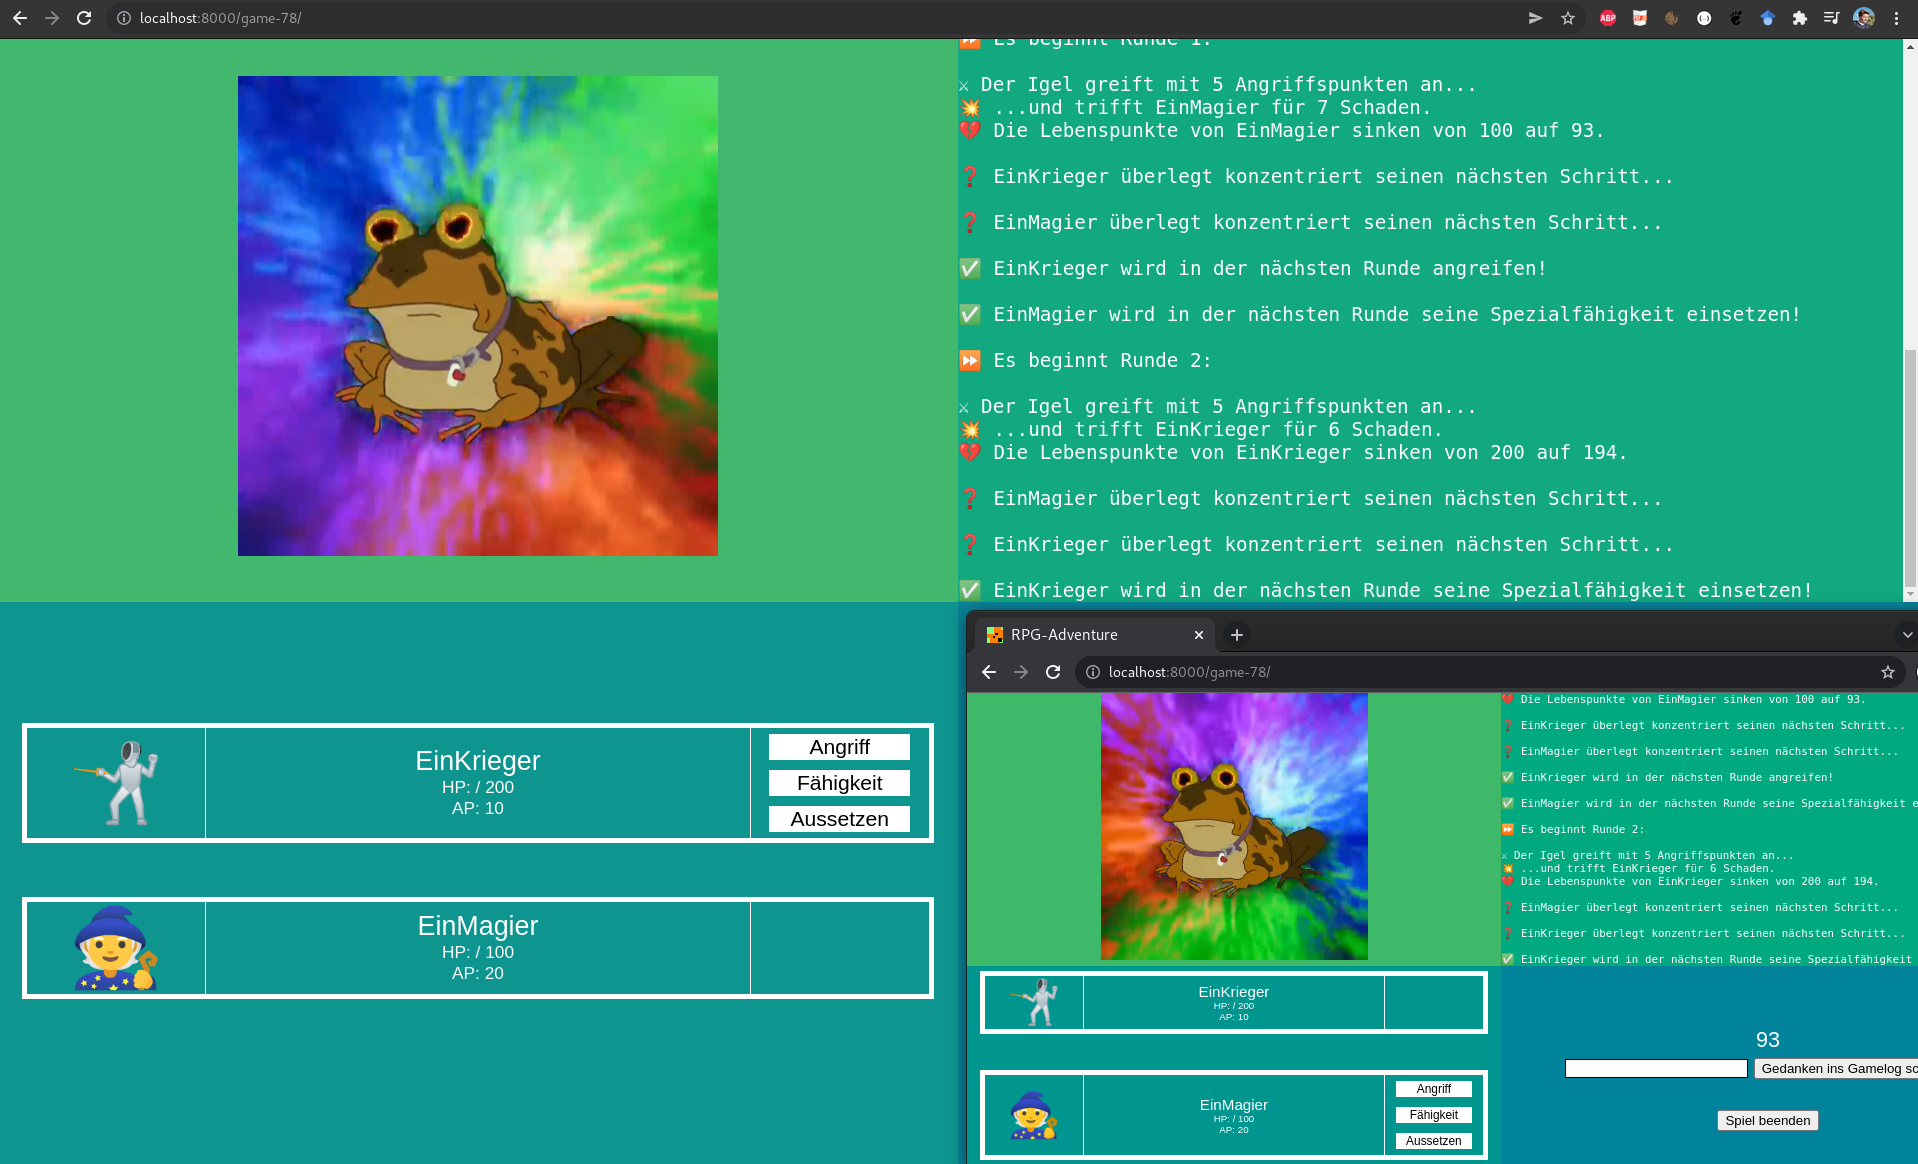
\includegraphics[width=0.7\textwidth]{2021-12-29-Bildschirmfoto-Entwicklungsstand-Runden-Status-400.png}
    \end{figure}

    \item Die Chatfunktion wurde implementiert. Hier jedoch abweichend vom Plan direkt als Meldungen im Game-Log und nicht in einem gesonderten Chat-Log und Chat-Fenster. Julian war damit im kurzen Teams-Gespräch gestern einverstanden. Den Aufbau der Game-Seite entsprechend angepasst und dem Game-Log deutlich mehr Raum eingeräumt. Außerdem weitere Anpassungen am Design und Style (Commit \url{https://git.io/JyDRK}).

\end{itemize}


\textbf{Entwicklung, Donnerstag 30.12.2021:}

Abschließender Schritt in der Implementation der Rundenlogik:

\begin{itemize}
    \item Die Schadensfunktion für Spieler wurde eingebaut: Damit kann dem Gegner nun Schaden zugefügt werden. Außerdem Prüfung auf Tod des Gegners incl. entsprechender Medlung (Commit \url{https://git.io/Jy9E7}).
\end{itemize}

Offen sind nun als nächste Schritte noch:
\begin{enumerate}
    \item Fähigkeiten der Spieler in Rundenlogik implementieren.
    \item Abschlussbildschirm für Sieg und Gameover konzeptionieren und implementieren. 
    \item Charakterentwicklung bei Sieg implementieren.
    \item Erweiterung der Infrastruktur aus Scripten, Anleitungen und des Git-Repos hin zum laden eines Default-Datensatzes (JSON-Datei) mit nutzbaren Spieldaten (insbesondere für Testzwecke und Nutzungen durch Dritte).
\end{enumerate}


\textbf{Entwicklung, Freitag 31.12.2021:}

Abarbeiten der zuletzt genannten, nächsten Schirtte. Hier: 

\begin{itemize}
    \item Die Charakterentwicklung wird mit Erfahrungspunkten gelöst: Durch Aktionen im Spiel bzw. Kampf (Schaden bekmmen, Schaden austeilen, Fähigkeiten nutzen) bekommen die entsprechenden Charaktere sofort entsprechende Erfahrungspunkte gutgeschrieben. Wird das Spiel gewonnen, werden alle von allen teilnehmenden Spielern in dieser Runde erspielten Erfarungspunkte noch einmal verdoppelt und jedem der Spieler gutgeschrieben. Verwendet werden können diese Erfahrungspunkte dann in der Charakteransicht um damit z.B. Lebenspunkte (HP) oder Angriffspunkte (AP) zu erhöhen (Commit \url{https://git.io/Jy7gl}).
\end{itemize}


\textbf{Entwicklung, Samstag 01.01.2022:}

Nach kurzer Abstimmung und Vorstellung meiner Ergebnisse bei Julian, letzte Anpassungen bzw. Entwicklungen: 

\begin{itemize}
    \item Ausgabe der erhaltenen XP beschleunigt: Es werden nun immer 10\% (aufgrundet auf die nächste Ganzzahl) der XP ausgegeben (Commit \url{https://git.io/JSTIq}).
    \item Einbau der Charakter-Fähigkeiten (Commit \url{https://git.io/JSkKJ}):
    \begin{itemize}
        \item Priester: Gruppe heilen=Alle HP erhöhen
        \item Zauberer: Schaden der Gruppe erhöhen=Alle AP erhöhen
        \item Krieger: Gegner blocken=AP Gegner verringern
    \end{itemize} 
    Damit die Fähigkeiten über mehrere Runden wirken können, musste eine Hilfstabelle angelegt werden: "AbilitysToApply". Hieraus werden zum Rundenwechsel die jeweils anzuwendenden Fähigkeiten gelesen und auf die relevaten Zahlen gewirkt. 
    \item Beispieldaten hinzugefügt und automatisches laden in die Datenbank über die local/dev-Skripte eingefügt (Commit \url{https://github.com/tstsrv-de/rpg/commit/1bfa99e89ddf2dbe817bdee2c870d1ddbe4f23c1}).
\end{itemize} 


\textbf{Entwicklung, Sonntag 02.01.2022}

Ein kurzer Anwendungstest mit einem versierten RPG-Spieler und IT-affinen Nutzer. Notizen dazu: 

\begin{itemize}
    \item Hinweis beim betreten der Lobby, dass das Spiel erst startet, wenn man einen "Platz-belegt" hat: Sofort erledigt!. 
    \item Man versuchte die Interaktion mit dem Spiel per Textkommandos über die Chatzeiel. Ineteresannte Alternative zur Nutzng der Buttons: Üübertragen in Ausblick(\ref{ausblick}). 
    \item Der erste Level ist mit über 10 Runden deutlich zu lang und muss verkürzt werden: Sofort erledigt!
\end{itemize}

Weiter wurden alle im Code enthaltenen Variablen und Konstanten in die Datenbank ausgelagtert. Dazu wurde eine neue Tabelle "MyRpgConfig" angelegt, alle Werte dorthin transportiert und im Code enstprechende Abfragen sowie weitergehende Anpassungen (z.B. Schleifen x-Fach durchlaufen) vorgenommen. Auch wurden die Beispiel- bzw. nun Basisdaten für die Datenbank entsprechend erweitert (Commits \url{https://git.io/JSGJD} und \url{https://git.io/JSGJ7}).


\textbf{Entwicklung, Sonntag 09.01.2022}

Nach letzter Projektbesprechung\ref{fig:2022-01-06-Projektbesprechung} in der vorallem Deatils zum weitern Ablauf, Meiliensteinen und zeitlichen Fristen besprochen wurden, kommen nun erste konkrete Texte zum Spiel-Inhalt. Dazu wurde das Spiel erweitert: Der bisherige Introtext ergänzt um eine Begrüßung durch den Gegener, sowie 2 Varianten (Gameover und Win) zum Spielende (Commit \url{}).

